\subsubsection{Página inicial do painel do aluno}
\label{ssub:student_dashboard}

Esta página é dirigida aos alunos autenticados, e é a primeira página que estes consultam após o registo ou autenticação.

Como é a primeira página consultada, pretende-se colocar as ações mais importantes e frequentes em todo o processo de gestão de projetos e unidades curriculares por parte do utilizador.\\

Optou-se assim por num plano principal colocar informação relativa a projetos, que se considera a informação mais relevante do sistema. Dividiu-se assim os projetos em três categorias distintas, os projetos ativos, os próximos e os terminados.

Os projetos ativos, são os projetos mais importantes para o utilizador, e por isso aparecem primeiro. Ao listar os projetos optou-se por colocar informação relativa à unidade curricular, data da próxima entrega e progresso.

De seguida lista-se os próximos projetos, onde colocou-se informação relativa à unidade curricular, data de inicio e primeira entrega.

Por fim, são listados alguns dos últimos projetos já terminados, com informação relativa à unidade curricular, data de fim e classificação obtida.

Ao carregar num projeto o aluno será direcionado para uma página com todas as informações deste.\\

Na barra da direita o aluno poderá ainda consultar as últimas notificações dos projetos das suas unidades curriculares, assim como consultar as unidades curriculares onde tem inscrição válida.
Ao carregar numa notificação o aluno é direcionado para a página do respetivo projeto.\\

Nesta página foram tidos todos os cuidados para selecionar a informação e as ações mais pertinentes para o utilizador, para permitir que este consulte com facilidade a informação que pretende, e para ajudar a manter o seu processo de gestão de trabalhos mais organizado.\\

Na Figura~\ref{fig:student_dashboard} pode ser consultada uma imagem demonstrativa da página desenvolvida.

\begin{figure}[H]
  \centering
  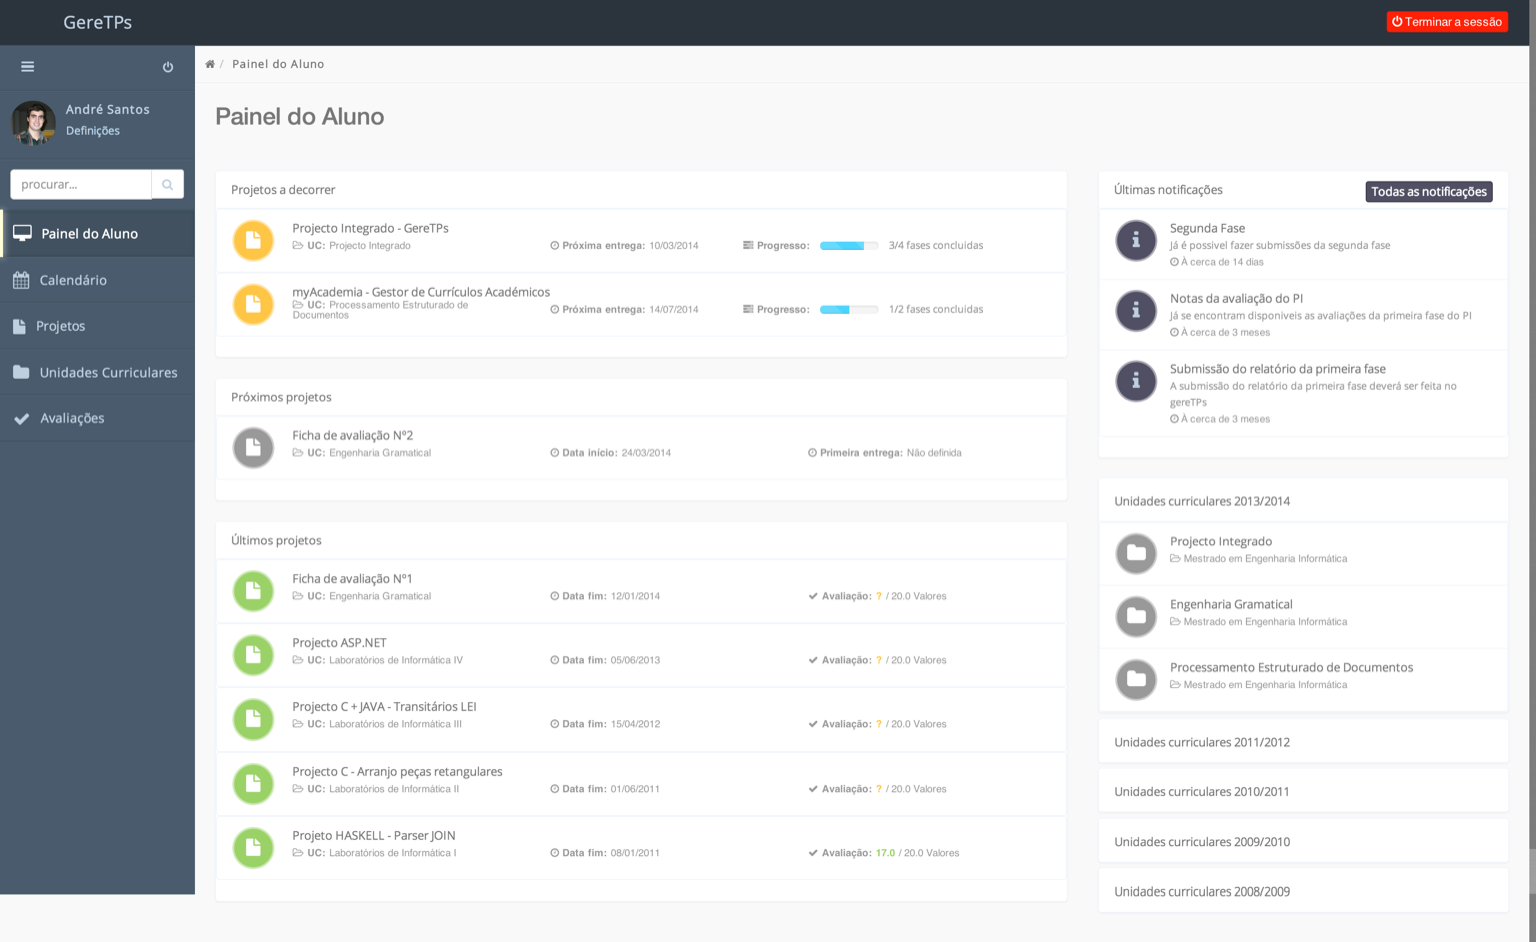
\includegraphics[width=1\textwidth,center]{images/implementacao/alunos/dashboard}
  \caption{Página inicial do painel do aluno}
  \label{fig:student_dashboard}
\end{figure}
